% Created 2024-10-27 Sun 21:18
% Intended LaTeX compiler: pdflatex
\documentclass[11pt]{article}
\usepackage[utf8]{inputenc}
\usepackage[T1]{fontenc}
\usepackage{graphicx}
\usepackage{longtable}
\usepackage{wrapfig}
\usepackage{rotating}
\usepackage[normalem]{ulem}
\usepackage{amsmath}
\usepackage{amssymb}
\usepackage{capt-of}
\usepackage{hyperref}
\usepackage{amsmath}
\author{Kristofer Čepon Povšič}
\date{\today}
\title{Holografija}
\hypersetup{
 pdfauthor={Kristofer Čepon Povšič},
 pdftitle={Holografija},
 pdfkeywords={},
 pdfsubject={},
 pdfcreator={Emacs 29.4 (Org mode 9.7.11)}, 
 pdflang={English}}
\begin{document}

\maketitle
\tableofcontents

\section{Uvod}
\label{sec:org072c4ed}

Holografija je vrsta fotografije, pri kateri ponazorimo predmet v treh dimenzijah.

Pri navadni fotografiji na fotografski film (oz. detektor) zabeležimo projekcijo porazdelitve gostote svetlobnega toka, ki ga seva predmet. Projekcija je dosežena s pomočjo optične leče in slika je dvodimenzionalna.

Svetlobno valovanje (električna poljska jakost) nosi podatek o globinski porazdelitvi posameznih točk na površini predmeta v fazi valovanja. Pri normalni fotografiji izgubimo podatek v fazi, ker je počrnitev film sorazmerna povprečni vrednosti kvadrata električne poljske jakosti. Pri hologramu podatke o fazah ohranimo tako, da na fotografsko ploščo posnamemo interferenčno sliko med svetlobo, ki jo siplje predmet in svetlobo, ki na poti do fotografski plošči predmet obide.

Kot izvor svetlobe uporabimo laser, saj je za doseg interference potrebno, da je koherentna dolžina svetlobe daljša od razlike poti, ki jo opravita predmeti in referenčni snop.

Električno poljsko jakost prepuščenega \(E_p\) in referenčnega žarka  \(E_r\) zapišemo kot

\begin{align*}
  E_p &= E_{p0}(x, y) e ^{- i \phi (x, y) } e ^{i \omega t} \\
  E_r &= E_{r0} (x, y) e ^{- i \psi (x, y)} e ^{i \omega t}
\end{align*}

kjer sta \(\phi, \psi\) fazi valovanja in je izhodišče koordinatnega sistema postavljeno tako, da se ravnina \((x, y)\) ujema s fotografsko ploščo.

Ker sta valovanji koherentni (torej lahko interferirata) velja:

\[ E(x, y) = E_p (x, y) + E_r (x, y)
\]

Ustrezna gostota svetlobnega toka \(I\) je sorazmerna kvadratu električne poljske jakosti

\begin{equation}
\label{eq:1}
I = (E_p + E_r) (E_p + E_r)^{*} = \left| E_p \right| ^2 + \left| E_r \right| ^2 + E_p E^{*}_r + E_p^{*}E_r
\end{equation}

Iz zadnjih dveh členov vidimo, da se na fotografsko emulzijo zapišeta tudi interferenčna člena, ki nosita informacijo o relativni fazi med snopoma.

Ploskovna gostota energije (ekspozicija) \(W_{ex}\) je enaka produktu gostoti svetlobnega toka \(I\) in času osvetljevanja \(t\).

Transmitivnost emulzije \(T\) je odvisna od ekspozicije \(W_{ex}\) podana z

\[ T \propto W_{ex}^{\gamma}
\]

kjer je parameter \(\gamma\) odvisen od lastnosti emulzije in načina razvijanja.

Definiramo amplitudno prepustnost definirano kot
\begin{equation}
\label{eq:2}
T_{ampl} = \sqrt{T}
\end{equation}

Pri upoštevanju \(E_p \ll E_r\) vstavimo \ref{eq:1} v \ref{eq:2} dobimo

\begin{equation}
\label{eq:3}
T_{ampl} = C \left| E_r \right| ^{\gamma} \left( 1 + \frac{\gamma}{2 \left| E_r \right|} (E_p E^{*}_r + E_p^{*}E_r) \right) = A + BE_p E^{*}_r + BE_p^{*}E_r
\end{equation}

kjer sta \(A, B\) konstanti.

Če hologram postavimo na prejšnje mesto, in ga osvetlimo z referenčnim žarkom, predmet pa odstranimo.

Na izstopni strani strani fotografske plošče je električna poljska jakost \(E_{holo}\) enaka produktu

\begin{equation}
\label{eq:4}
E_{holo} = T_{ampl} \cdot E_r =  AE_r + BE_p \left| E_r \right| + BE_p^{*}E_r^2
\end{equation}

Prvi člen predstavlja delno prepuščeni referenčni žarek. Drugi člen opisuje divergenten žarek, ki je tako kot da bi izviral iz predmeta in v očesu ustvari virtualno sliko predmeta na originalnem mestu, kjer smo ga slikali.
Tretji člen opisuje konvergentni žarek, ki daje realno sliko predmeta in je opazen npr. na drobnih delcih cigaretnega dima. Do tega pridemo, če \ref{eq:4} pomnožimo z \(E_r^{*}\).

Postavitev za predmet je taka kot na sliki \ref{fig:1}

\begin{center}\label{fig:1}
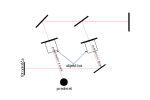
\includegraphics[width=.9\linewidth]{predmet.pdf}
\end{center}
\subsection{Hologram ravnih valov}
\label{sec:org2e856b7}

Sedaj imejmo predmetni in referenčni žarek kot ravna valova oblike \(e^{i(kr - \omega t)}\), prvi pod kotom \(\alpha\) na fotografsko ploščo in drugi v smeri normale. Izberimo si koordinatni sistem tako, da lahko žarka zapišemo kot \(\vec{k_p} = (k \sin \alpha, 0, k \cos \alpha)\) in \(\vec{k_r} = (0, 0, k)\).
Fotografska plošča se nahaja v ravnini \(z = 0\). Potem je intenziteta interferenčnega vzorca na njej enaka

\begin{equation}
\label{eq:5}
I_{int} = C \left| 1 + e^{ik \sin \alpha x} \right| ^2 = C' (1 + \cos(k\sin \alpha x))
\end{equation}

Hologram je kosinusna uklonska mrežica s periodo

\begin{equation}
\label{eq:6}
d = \frac{2 \pi}{k \sin \alpha}
\end{equation}

Natačnejši račun s Fraunhoferjevim uklonskim integralom bi nam pokazal, da dobimo pri osvetltvi kosinusne uklonske mrežice z ravnim valom poleg prepuščenega vala še dva uklonjena žarka prvega reda, ki sta razporejena simetrično levo in desno glede na prepuščeni val.

Splošen tankoplastni hologram lahko torej razumemo kot superpozicijo kosinusnih uklonskih mrežic, ki nastanejo pri interferenci referenčnega žarka in žarkov, ki izvirajo iz posameznih točk objekta.

Postavitev za ravne valove pa je na sliki \ref{fig:2}

\begin{center}\label{fig:2}
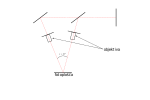
\includegraphics[width=.9\linewidth]{ravni_zarek.pdf}
\end{center}
\section{Potrebščine}
\label{sec:orgc1ffef0}

\begin{itemize}
\item He-Ne laser ( \(\lambda = 623.8 \mathrm{nm}\) )
\item dve zrcali
\item dve leči
\item delilnik žarka
\item fotografska plošča
\item predmet
\end{itemize}
\section{Naloge}
\label{sec:org93ee1e7}
\begin{itemize}
\item sestavi postavitev za snemanje holograma in ga posnemi
\item posnemi interferogram dveh ravnih valov
\end{itemize}
\section{Navodila}
\label{sec:org9ab1b67}

Laserski snop s pomočjo delilca razdelimo na dva žarka, ki ju razpršimo z mikroskopskima objektivoma. Naredimo predmetni žarek, ki osvetli predm in referenčni žarek, ki predmet obide. Pravilno ju usmerimo z zrcali.

V drugem delu vaje je postavitev nekoliko drugačna. Postavimo oba snopa enega vzporedno na normalo fotografske plošče in drugega pod nekim kotom \(\alpha\). Tako lahko postavimo interferogram.

V tri banjice pripravimo razvijalec, vodo in fiksir za razvijanje slike, s katerimi potem razvijemo hologram.
\section{Meritve}
\label{sec:org1bd5112}

Tekom vaje sem postavil in uspešno tudi posnel hologram predmeta.

Glej sliko \ref{fig:3}

\begin{center}\label{fig:3}
\includegraphics[width=.9\linewidth]{20241015_131245(1).jpg}
\end{center}

Prav tako sem uspel posneti tudi interferogram, kjer sem izmeril sledeče podatke:

\begin{align} \label{al:1}
a &= 94 mm \pm 0.1 mm \\
x &= 255 mm \pm 0.5 mm
\end{align}
\section{Izračuni}
\label{sec:org51bb9fd}

Po formuli

\begin{equation}
\label{eq:7}
\sin \alpha = \frac{x}{a}
\end{equation}

izračunamo \(\alpha = 0.38 \pm 0.02\) in nato uporabimo izraz \ref{eq:6} in vrednost valovne dolžine našega laserja He-Ne, da dobimo vrednost

\[
d = (2.33 \pm 0.05) \mu m
\]
\end{document}
